% Chapter Template
% cSpell:words parencite 
\chapter{Marco teórico} % Main chapter title 

\label{Chapter2} % Change X to a consecutive number; for referencing this chapter elsewhere, use \ref{ChapterX}
En este capítulo se comprenderán conceptos teóricos sobre las tecnologías claves en las cuales se basa el proyecto. Como introducción, se analizará el funcionamiento de las redes tradicionales, donde se dejará en evidencia la necesidad de un nuevo paradigma. 

Luego, se analizarán los fundamentos en los que se basan las Redes Definidas por Software y por qué este paradigma resuelve los problemas presentados por el enfoque de las redes tradicionales. 

También, se introducirán conceptos de lenguajes de modelado y se abordará la importancia de la gestión de la red. Se estudiará \textit{NETCONF} como protocolo de gestión de red. Finalmente, se abordan conceptos de dispositivos ópticos de transporte.

%----------------------------------------------------------------------------------------
%	SECTION 1
%----------------------------------------------------------------------------------------
\section{Redes tradicionales} \label{sec:rdtr}

La infraestructura actual de las redes tradicionales basan su funcionamiento íntegramente en los dispositivos de red. Cada dispositivo lleva su propia gestión sobre el plano de datos y el plano de control de manera local y comunica a los demás dicha información de ser necesario. 

Un ejemplo de esto se puede observar en la figura \ref{fig:dev_tradicional}, donde dos dispositivos intercambian información referente al plano de control.
\\

\begin{figure}[htbp]
	\centering
	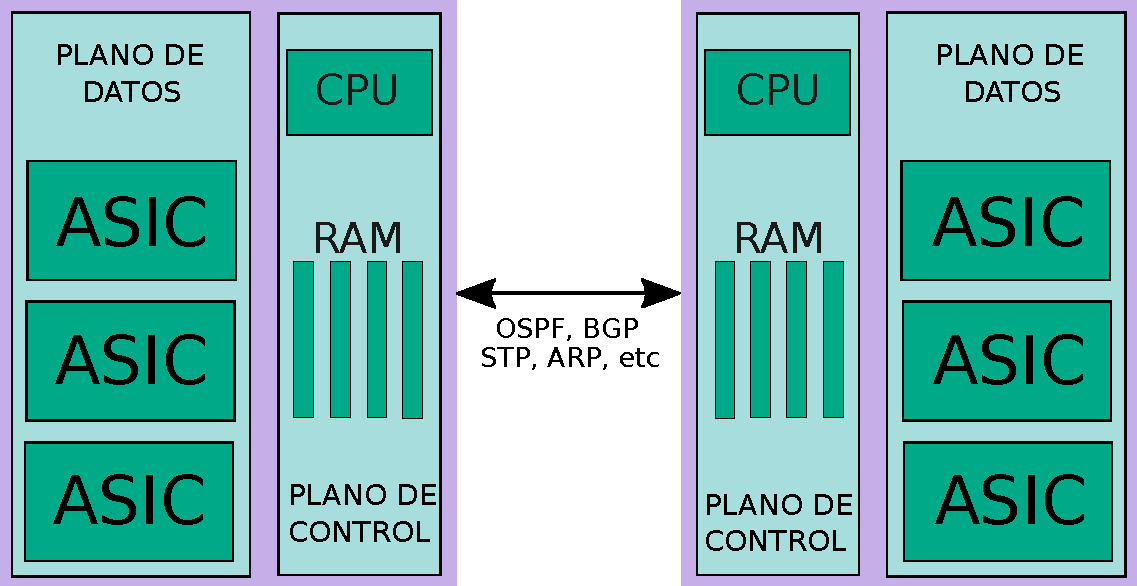
\includegraphics[scale=0.6]{Figures/dispositivo-tradicional.pdf}
	\caption{Comportamiento de dispositivos en redes tradicionales.}
	\label{fig:dev_tradicional}
  \end{figure}


\subsection{Plano de Control}
Comprende la configuración del sistema, la administración y el intercambio de información de ruteo entre los dispositivos. Es el responsable de administrar la configuración del equipo y de programar el camino que será usado para el flujo de los paquetes. En otras palabras, es en este plano donde se calculan y se toman las decisiones de enrutamiento y reenvío. En las redes tradicionales, cualquier aplicación que utilice el dispositivo para administrar su configuración reside en esta capa. 

El proceso de establecimiento de la topología de red utilizando un plano de control que se ejecuta localmente, es compleja debido a que no existe ningún dispositivo que sea conocido por toda la red. Para gestionar cambios o actualizaciones en cada dispositivo se debe estar conectado a su plano de control de forma individual, lo que no resulta en un enfoque inteligente.

\subsection{Plano de Datos}
También conocido como plano de usuario o plano de reenvío, es el encargado de transportar el tráfico de usuario hacia el destinatario final. Una diferencia importante que tiene el tráfico correspondiente al plano de datos con respecto al plano de control, es que el primero es generado en los terminales mientras que en el segundo caso, el tráfico es generado en los dispositivos de red. Tiene como objetivo el reenvío de los paquetes hacia el próximo salto basándose en las decisiones tomadas por la capa de control.
\\


El enfoque dado por las redes tradicionales cumplió con las necesidades de una época donde las arquitecturas cliente-servidor eran dominantes. Tiene como ventaja ser simple a nivel lógico, mientras que el plano de control implica el uso de microprocesadores para tratar los paquetes y conformar las tablas, el plano de datos se desarrolla en silicio. A pesar de ello, presenta una serie de problemas:

\begin{itemize}
	\item \textbf{Funcionalidad de la red integrada en los dispositivos:} El plano de control se encuentra íntegramente en los dispositivos de red, lo que resulta en una configuración de red estática, inflexible y descentralizada. 
	\item \textbf{Escalabilidad:} La escalabilidad resulta afectada y no apropiada para la explosión de las nuevas tecnologías como \textit{Big Data}, \textit{Cloud Computing} y el \textit{Streaming}, donde la complejidad de la red incrementa rápidamente debido a que cada dispositivo agregado debe ser configurado y administrado.
	\item \textbf{Políticas inconsistentes:} Si las políticas de configuración cambian a nivel de red, implica un cambio en todos los dispositivos que la componen por parte de los administradores de red.
	\item \textbf{Dependencia del fabricante y personalización:} El plano de control integrado a los dispositivos de red resulta en una dependencia a los ciclos de producción de equipamientos por parte de los fabricantes para incorporar nuevas funcionalidades. Además, con la finalidad de asegurar la calidad de servicio y brindar alta perfomance, la industria define los protocolos de red de forma específica y aislada, sin el beneficio de una acción conjunta e incapacitando a los operadores a personalizar la red para sus entornos individuales y específicos. 
\end{itemize}

%----------------------------------------------------------------------------------------
%	SECTION 2
%----------------------------------------------------------------------------------------
\section{Redes Definidas por Software} \label{sec:rsdn}

A diferencia de las aplicaciones y los nuevos requerimientos de los usuarios, las redes no han cambiado mucho respecto a los últimos 30 años. El desarrollo de las \textit{SDN} se inició en 1990 donde se introdujo el concepto de funciones programables en la red, teniendo gran innovación en 2001-2007 donde se propone separar el plano de datos del plano de control. El próximo gran paso de las \textit{SDN} llegó en 2007-2010, con la implementación de la \textit{API OpenFlow}.

Las redes definidas por software nacen en respuesta a la dinámica y flexibilidad que requieren las nuevas tendencias, donde el enfoque presentado por las redes tradicionales no cumple dado su naturaleza estática. 

\subsection{Definición de \textit{SDN}}
Según la \textit{ONF}, la red definida por software, también conocida como red programable o automatizada, consiste en una arquitectura donde el plano de datos se encuentra separado del plano de control y donde este último a su vez puede controlar varios dispositivos.

Este nuevo paradigma presenta las siguientes ventajas:

\begin{itemize}
	\item \textbf{Plano de control centralizado:} A diferencia del enfoque presentado por las redes tradicionales donde se tenía un plano de control distribuido entre los diferentes equipos que conforman la red, ahora se tiene un plano de control centralizado y presente a nivel lógico en un mismo punto. De esta forma, se tiene una visión general y global de toda la red, relajando las comunicaciones entre los dispositivos y las complejidades introducidas por las configuraciones individuales de cada uno. Además, el plano de control ahora es directamente programable, sin tener que usar como intermediario el plano de datos. Todo el tráfico ahora está bajo la supervisión de este nuevo plano de control centralizado, transformando a la red en una red programable. 
	\item \textbf{Costos:} Los costos relacionados al control de la gestión del tráfico y de configuración de los diferentes equipos se ven reducidos en tiempo y esfuerzo dado el plano de control centralizado.
	\item \textbf{Automatización:} Un beneficio indirecto de tener un plano de control centralizado, es poder tomar diferentes decisiones y políticas en base a la visibilidad global de la red en tiempo real, aplicando configuraciones en los diferentes equipos de forma automática.
	\item \textbf{Escalabilidad:} \textit{SDN} admite topologías dinámicas con capacidades para adaptarse a cambios, debido a la automatización de la configuración de los dispositivos. Con la capacidad de ajustar los picos y las bajas en la carga del tráfico, las empresas pueden crear e implementar nuevos servicios y aplicaciones sin demora debido a la infraestructura más flexible.
	\item \textbf{Mantenimiento y monitoreo:} Por medio del controlador \textit{SDN} se puede conocer, en cualquier momento, el estado actual de la red incluyendo los dispositivos que la componen.
	\item \textbf{Seguridad:} Dado que la administración de toda la red se realiza en un solo punto, se asegura que no existan debilidades o inconsistencias en las configuraciones de las aplicaciones y los equipos.
\end{itemize}

\subsection{Arquitectura de \textit{SDN}}
En las redes tradicionales, cada dispositivo tiene integrado tanto el plano de datos como el plano de control. En \textit{SDN}, el plano de datos se encuentra desacoplado del plano de control y, además, se puede diferenciar un nuevo plano llamado \textit{plano de aplicación}. A continuación, se analizará cuál es la función que cumple cada plano en esta nueva arquitectura propuesta por las \textit{SDN}.

\subsubsection{Plano de Datos}
Comprende la misma funcionalidad que en las redes tradicionales. Consiste en un conjunto de dispositivos de red con funcionalidades de reenvío de paquetes.

\subsubsection{Plano de Aplicación}
Con el enfoque de las redes tradicionales, el plano de aplicación se encontraba integrado en el plano de control. En \textit{SDN}, el plano de aplicación se desacopla al igual que el plano de control. En este plano se encuentran las aplicaciones de red que implementan las funcionalidades de más alto nivel y que participan en las decisiones de administración y control de ruteo.

\subsubsection{Plano de Control}
Toda la función de control se encuentra centralizada fuera de los dispositivos, permitiendo a los desarrolladores de aplicaciones utilizar las capacidades de la red pero haciendo una abstracción de su topología o sus funciones. Tiene como objetivo mediar, organizar y facilitar la comunicación entre los diferentes equipos y las aplicaciones. Además, este plano ahora está disponible para poder ser programado desde un software externo al controlador.

En la figura \ref{fig:arquitectura_sdn}, , se expone la anatomía de un controlador \textit{SDN}. En ella, se puede observar dos interfaces comprendidas por el plano de control: \textit{Southbound} y, \textit{Northbound}.

\begin{itemize}
	\item \textbf{\textit{Southbound API}:} necesaria por la separación del plano de control del plano de datos. Define la \textit{API} de comunicación entre el controlador y los diferentes dispositivos de red, en otras palabras, entre el plano de control y el plano de datos.  
	\item \textbf{\textit{Northbound API}:} funciona como interfaz tanto de alto como de bajo nivel, es necesaria para permitir que las aplicaciones que se ejecutan en la parte superior de \textit{SDN} puedan comunicarse con el mismo. En el primer caso, la interfaz provee una abstracción de la red en sí misma, permitiendo a los desarrolladores no tener que preocuparse por los dispositivos individuales, sino manejar la red como un todo. En el segundo caso, la interfaz advierte a las aplicaciones sobre la existencia de los dispositivos individuales y sus enlaces, pero oculta las diferencias entre los dispositivos. 
\end{itemize}


\begin{figure}[htbp]
	\centering
	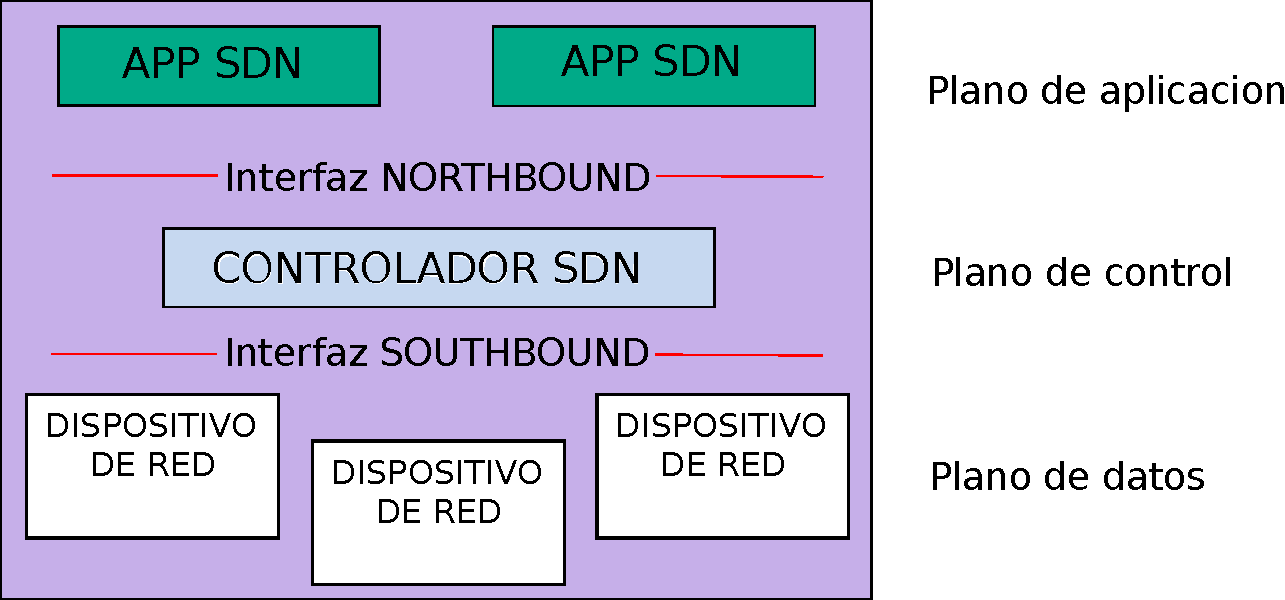
\includegraphics[scale=0.5]{Figures/arquitectura-controlador.pdf}
	\caption{Arquitectura de un controlador \textit{SDN} tradicional.}
	\label{fig:arquitectura_sdn}
  \end{figure}

%----------------------------------------------------------------------------------------
%	SECTION 3
%----------------------------------------------------------------------------------------
\section{Gestión de la Red} \label{sec:gestionred}
En la actualidad se puede encontrar una gran variedad de redes, desde pequeñas redes domésticas de intranet hasta redes empresariales o de proveedores de servicios. Cada una de estas redes tienen diversos requerimientos de gestión.  Las pequeñas redes domésticas, que consisten en unos pocos dispositivos conectados, requieren una sobrecarga de administración baja, y con frecuencia, pueden gestionarse manualmente de forma eficiente. No así las redes más grandes, que podrían contener cientos dispositivos conectados requiriendo un enfoque más sistemático para hacer frente a las complejidades que surgen debido al tamaño de la red. A medida que la red crece en estructura y complejidad, se hace evidente la necesidad de una solución eficiente para la gestión de la misma.

\subsection{Protocolos de Gestión}
Existen múltiples formas de llevar a cabo la administración de la configuración en los diversos dispositivos que conforman la red. En esta sección, se analizarán dos alternativas: \textit{CLI} y \textit{SNMP}.

\subsubsection{Command Line Interface}
\textit{CLI} es el enfoque más común en el ámbito de gestión de la configuración, adoptado por múltiples empresas. Está orientado a que resulte fácil de entender para las personas, presentando una interfaz de texto simple. Sin embargo, no se encuentra orientado a las \textit{API’s}, donde la implementación interna podría ser diferente entre los distintos dispositivos, incluso entre dispositivos del mismo fabricante. La \textit{CLI} puede utilizar \textit{API’s} internas para cambiar la lógica de la función de red o bien podría transformar los comandos ingresados en un archivo de configuración y reiniciar la configuración del dispositivo con dicho archivo.

\newpage
Un ejemplo de una operación en \textit{CLI} puede verse en la figura \ref{fig:cli}
\\
\begin{figure}[htbp]
	\centering
	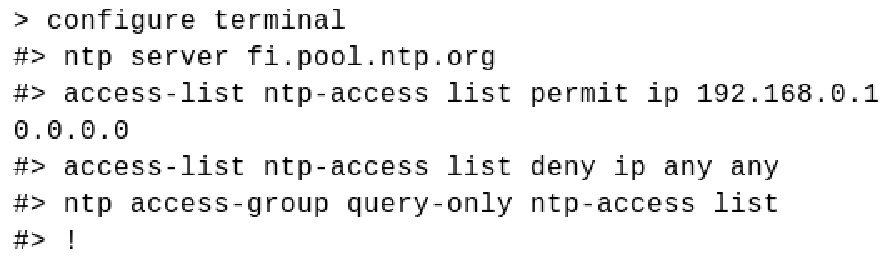
\includegraphics[scale=0.6]{Figures/cli.pdf}
	\caption{Interaccion tipica con un dispositivo mediante \textit{CLI}.}
	\label{fig:cli}
  \end{figure}

  Este enfoque presenta una serie desventajas. En primer lugar, la implementación de las API’s \textit{CLI} no están estandarizadas, por lo que las operaciones varían drásticamente entre dispositivos de diferentes fabricantes e incluso en implementaciones \textit{CLI} del mismo fabricante. A su vez, los fabricantes podrían brindar una actualización de software del dispositivo donde los comandos \textit{CLI} de la versión anterior se vean modificados o eliminados, lo que no solo se traduce a problemas para el administrador de red, sino también para las API que usen la \textit{CLI}. En segundo lugar, algunas operaciones en la gestión de la configuración podrían requerir múltiples transacciones \textit{CLI}, si alguna de estas transacciones falla, el dispositivo podría quedar en un estado inconsistente. \textit{CLI} no define de forma estándar una solución para deshacer los cambios aplicados en el dispositivo.

  \subsubsection{Simple Network Management Protocol}
  \textit{SNMP} es un protocolo de monitoreo y administración de red, estandarizado por primera vez en 1988 por la \textit{IETF}. Su funcionamiento se basa en una arquitectura cliente-servidor, donde los mensajes se intercambian a través del protocolo de transporte no orientado a la conexión \textit{UDP}. Consiste en una colección de agentes y administradores formando entre ellos una red, donde se denomina administrador a aquel dispositivo que tiene el rol de ejecutar aplicaciones de administración de red, mientras que los dispositivos que requieran ser administrados se denominan agentes.

  Las capacidades para administrar la red en \textit{SNMP} quedan representadas en lo que se conoce como \textit{MIB}. Una \textit{MIB} es una base de datos que contiene información jerárquica y estructurada en forma de árbol de todos los parámetros gestionables de la red. 
  Dicha base de datos se debe cargar en el administrador \textit{SNMP}, para ello cada agente \textit{SNMP} expone al administrador \textit{SNMP} una serie de módulos \textit{MIB}. Con esta información el administrador podría alterar dinámicamente la configuración del agente. 
  \\
  El uso de \textit{SNMP} como monitoreo es una práctica común desde su publicación, sin embargo, se desalentó su uso en áreas de gestión de configuración por las siguientes razones: 

  \begin{itemize}
	\item Problemas inherentes al protocolo de transporte \textit{UDP}, donde los mensajes pueden perderse o llegar desordenados, así como también la falta de mecanismos de seguridad para los mismos jugaron un papel importante para reemplazar \textit{SNMP} por otros protocolos de administración de red.
	\item No existe una estandarización de los módulos \textit{MIB} para configurar las funciones de red. El trabajo de descubrir correctamente los módulos \textit{MIB} para cada dispositivo es tarea del usuario, lo que resulta compleja y no eficiente.
\end{itemize}

\subsubsection{Otras alternativas}
Algunos enfoques para la gestión de la red pueden incluir soluciones basadas en páginas web, que permiten al administrador modificar las configuraciones en el dispositivo de forma gráfica y más amigable, pero generalmente resultan más limitadas que las \textit{CLI}. 
Además, algunos dispositivos pueden brindar soluciones propietarias para la gestión de la configuración, sin embargo, estas soluciones suelen ser muy específicas a un dispositivo o una familia de dispositivos, y rara vez suelen ser compatibles entre sí. Estos últimos también representan una carga para los administradores, donde cada solución requiere que el administrador aprenda otra manera de configurar las funcionalidades de la red.  

\subsection{\textit{NETCONF}}
Esta sección repasa brevemente los conceptos y características principales que ofrece el protocolo \textit{NETCONF}. Además, aspectos de seguridad, transporte y control de acceso del protocolo se discuten en detalle. 

\subsubsection{Definición}
\textit{NETCONF} fue estandarizado por la \textit{IETF} por primera vez en el 2006, en el \textit{RFC 4741}. Actualmente está siendo adoptado por los principales proveedores de dispositivos de red y ha ganado el apoyo de la industria. Según [], podemos encontrar que fabricantes como Juniper, Huawei, Cisco, entre otros, brindan soporte desde hace tiempo del protocolo \textit{NETCONF}. 
\\

La \textit{IETF} definde a \textit{NETCONF} como un protocolo estándar para \textit{Instalar, manipular y borrar configuraciones en un dispositivo}. Permite implementar una \textit{API} formal utilizando el lenguaje de modelado \textit{YANG} para administrar y monitorear las funcionalidades de la red. \textit{NETCONF} utiliza el paradigma de las \textit{RPC}, donde construye los mensajes que intercambian información como un flujo con codificación \textit{XML}. Funciona con una arquitectura cliente-servidor, donde los mensajes son transportados utilizando algún protocolo orientado a la conexión. El RFC 6241, en la sección 1.2, menciona una partición conceptual del protocolo en cuatro capas. La figura \ref{fig:netconf} detalla lo mencionado anteriormente. A continuación, se explica qué función cumple cada una de estas capas.

\begin{itemize}
	\item \textbf{Capa de transporte seguro:} provee mecanismos de comunicación entre cliente y servidor.  
	\item \textbf{Capa de mensajes:} encargada de la codificación y partición de los mensajes.  
	\item \textbf{Capa de operación:} define las operaciones admitidas por el protocolo.
	\item \textbf{Capa de contenido:} relaciona la representación y el modelado de los datos en el protocolo.    
\end{itemize}

\begin{figure}[htbp]
	\centering
	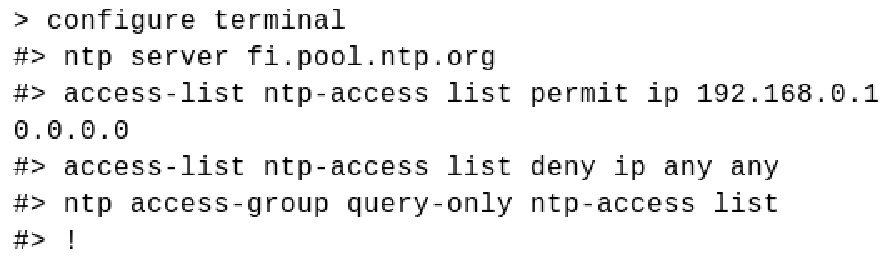
\includegraphics[scale=0.6]{Figures/cli.pdf}
	\caption{Separacion conceptual del protocolo NETCONF.}
	\label{fig:netconf}
  \end{figure}


  Las características que destacan a NETCONF como protocolo de administración de red son:

  \begin{itemize}
	\item Capacidad de restauración de los datos y backup de la configuración.
	\item De uso fácil, presentando la información de forma estructurada con una codificación entendible para las personas y las API’s.
	\item Implementa mecanismos de control de errores mediante validación de sintaxis y semántica.
	\item Separación clara de los datos de configuración y los datos de estado.
	\item Posibilidad de gestionar la configuración en un dispositivo de manera reactiva mediante notificaciones del mismo.
\end{itemize}

NETCONF separa los datos de configuración de los datos de estado de un dispositivo. Según lo detallado en la sección 1.1. y 1.4 del RFC6242, se define a cada uno como:

\begin{itemize}
	\item \textbf{Datos de configuración:} información que se puede leer o escribir y que se utiliza para llevar al dispositivo de un estado inicial a un estado deseado. Un ejemplo es la velocidad del ventilador del cpu del dispositivo.  
	\item \textbf{Datos de estado:} representa información de sólo lectura y estadísticas brindadas por el dispositivo. Por ejemplo, la temperatura del cpu del equipo.   
\end{itemize}

\subsubsection{Conceptos del Protocolo}
Como se mencionó anteriormente, NETCONF define un protocolo de administración de red con arquitectura cliente-servidor, donde el cliente en este caso es el sistema de administración de la red o el administrador del sistema, mientras que el dispositivo que contiene una o más funciones de red que deben ser administradas, actúa de servidor. El cliente y el servidor inician la sesión de protocolos mediante un primer mensaje que da lugar al intercambio de capacidades o \textit{capabilities}, donde se definen qué operaciones estarán disponibles para su uso. Este primer mensaje recibe el nombre de \textit{HELLO} [X]. La figura \ref{fig:netconf_comunicacion} refleja una comunicación típica entre un cliente y un servidor NETCONF.

\begin{figure}[htbp]
	\centering
	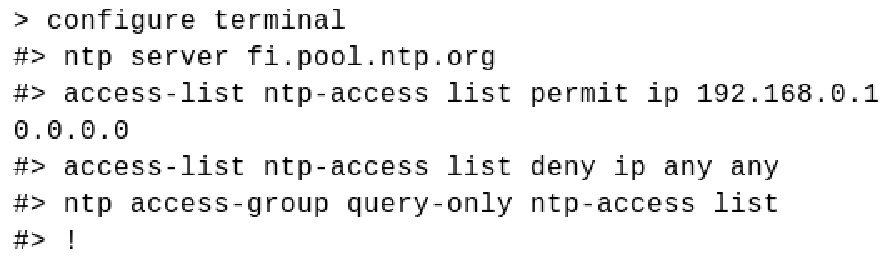
\includegraphics[scale=0.6]{Figures/cli.pdf}
	\caption{Comunicacion entre cliente y servidor NETCONF.}
	\label{fig:netconf_comunicacion}
  \end{figure}

  \subsubsection{Capacidades}
  El protocolo NETCONF está diseñado para ser altamente extensible y, con este fin, es compatible con el intercambio inicial de capacidades entre cliente y servidor. Este intercambio de información permite al cliente ajustar sus comportamientos basándose en las funcionalidades que admite el servidor. Cada capacidad recibe un nombre asignado por la \textit{IANA}, que indica las capacidades que no se pueden describir completamente utilizando únicamente \textit{YANG}. Por lo general, no es necesario agregar nuevas capacidades a NETCONF. 

  También incluye el intercambio de los modelos \textit{YANG} que tiene implementado el servidor, que es necesario no solo para que el cliente pueda aprender de los mismos, sino también para reconocer las diferentes revisiones implementadas en el servidor.

  \subsubsection{Sesión orientada a la conexión}
  La sección dos del RFC6242, referida a protocolos de transporte, detalla que NETCONF no esta vinculado a ningún protocolo de transporte específico. El requisito necesario de NETCONF para el protocolo de transporte subyacente es que el mismo sea orientado a la conexión. 

  \subsubsection{Sesión orientada a la autenticación}
  El protocolo NETCONF es orientado a la sesión con autenticación, utilizando una arquitectura cliente-servidor donde el servidor escucha un puerto asignado para recibir las conexiones con los clientes. 

  Según la sección dos del RFC6242 referida a seguridad, el protocolo mínimamente debe ofrecer autenticación, confidencialidad e integridad. Cualquier mensaje NETCONF, incluido el mensaje \textit{HELLO}, se envian unicamente si el cliente y servidor se han autenticado de forma correcta. No se especifica un protocolo en particular, pudiendo utilizarse alguno de los múltiples protocolos de transporte seguros existentes en la actualidad como \textit{TLS}, \textit{SSH}, \textit{BEEP}, etc. Cualquier implementación de NETCONF debe, al menos, soportar \textit{SSH} como protocolo de transporte seguro.

  Además, según el RFC6536 relacionado al control de acceso de usuarios, NETCONF admite una jerarquía de niveles de usuarios. Por ejemplo, tener dos grupos de usuarios donde uno tenga permisos de configuración más limitados que el otro.

  \subsubsection{Bases de datos}
  NETCONF define en la sección cinco del RFC6242, la existencia de uno o más datastores, los cuales cumplen el papel de una base de datos conceptual que puede ser utilizada para almacenar y acceder tanto a los datos de configuración como a los datos de estado. El protocolo especifica y define tres tipos de base de datos: \textit{startup}, \textit{running} y \textit{candidate}, de los cuales únicamente es obligatorio que se implemente \textit{running}. Si la implementación admite otras bases de datos, como por ejemplo \textit{startup} o \textit{candidate}, el servidor informará al cliente esta capacidad en el mensaje \textit{HELLO}. Cada operación en NETCONF debe especificar la base de datos a la cual realizará la consulta o modificación.
  \\

  A continuación, se detalla cada una de las bases de datos mencionadas.
\begin{itemize}
	\item \textbf{\textit{startup}:} según lo especificado en la sección 8.7 del RFC6242, dicha base de datos se utiliza para almacenar de forma persistente la información de configuración del dispositivo. El contenido de esta es copiado de manera automática a la base de datos conocida como \textit{running} en el inicio del servidor NETCONF. 
	\item \textbf{\textit{running}:} refleja la configuración actualmente en uso por el dispositivo. Es la unica base de datos conceptual que admite la presencia tanto de datos de estado como datos de configuración. 
	\item \textbf{\textit{candidate}:} se encuentra definido en la sección 8.3 del RFC6242. Puede ser utilizado para realizar cambios que no se van a aplicar al dispositivo de forma directa, sino que lo harán una vez se realice un \textit{commit} sobre dicha base de datos. De esta forma, el contenido de esta es copiado al \textit{datastore} running. Si de lo contrario se desea descartar los cambios realizados en este \textit{datastore}, la operación discard-changes copia el contenido del \textit{datastore} \textit{running} al \textit{datastore} \textit{candidate}. Únicamente se admite datos de configuración.
\end{itemize}


Como se mencionó anteriormente, cualquier implementación de NETCONF debe admitir al menos el \textit{datastore running}, esto es necesario ya que los datos de estado (necesarios para monitorear el dispositivo) únicamente se encuentran admitidos en dicho \textit{datastore}.

\subsubsection{Operaciones del protocolo}

Las operaciones en el protocolo NETCONF se definen como \textit{RPC} en los modelos \textit{YANG} relevantes. En dichos modelos también se definen los argumentos de entrada y los contenidos de salida para cada operación. Todas las operaciones están codificadas en \textit{XML} dentro de los mensajes \textit{RPC} que son, de hecho, los únicos mensajes que los clientes pueden enviar en las sesiones de NETCONF después del intercambio inicial del mensaje \textit{HELLO}. 

Como las operaciones son \textit{RPC}, cada mensaje enviado por los clientes tiene una respuesta por parte del servidor. Este resultado normalmente contiene \textit{ok} para indicar que la operación resultó según lo esperado, o \textit{error} indicando las razones por la cual falló dicha operación.
\\

El protocolo NETCONF define en la sección 7 del RFC6241 nueve operaciones básicas y necesarias para cualquier implementación del mismo, las cuales se describen a continuación:
\begin{itemize}
	\item \textbf{\textit{get}:} utilizado para consultar tanto datos de configuración como datos de estado al servidor NETCONF.
	\item \textbf{\textit{get-config}:} operación que devuelve los datos de configuración del servidor NETCONF. Puede incluir filtros para limitar la información enviada por parte del servidor.
	\item \textbf{\textit{edit-config}:} operación definida para crear, actualizar o borrar datos de configuración en el servidor NETCONF. Únicamente se admite esta operación en las bases de datos \textit{running} o \textit{candidate}.
	\item \textbf{\textit{copy-config}:} crea o reemplaza completamente el contenido de una base de datos por otra. El caso de uso más común de esta operación es para copiar el contenido del \textit{datastore running} al \textit{datastore startup}. 
	\item \textbf{\textit{delete-config}:} Elimina completamente el contenido de un \textit{datastore} determinado. No se admite esta operación para el \textit{datastore running}.
	\item \textbf{\textit{lock}:} permite al cliente bloquear la configuración completa de un \textit{datastore} específico en un dispositivo. Tales bloqueos son destinados a ser de corta duración, de esta forma un cliente puede realizar un cambio sin temor a la interacción con otros clientes de NETCONF. Además, como el protocolo es orientado a la sesión, todos los recursos tomados por la misma tales como los datastores, deben ser liberados en el momento de la finalización o cierre de la sesión.
	\item \textbf{\textit{unlock}:} permite a la sesión liberar el recurso tomado por la operación lock.
	\item \textbf{\textit{close-session}:} utilizada para finalizar la sesión entre cliente y servidor NETCONF. Cualquiera de las operaciones mencionadas en esta sección, quedan inhabilitadas una vez finalizada la sesión.
	\item \textbf{\textit{kill-session}:} permite al administrador de red finalizar alguna sesión inactiva que tiene recursos tomados. 
\end{itemize}

Además de estas nueve operaciones descritas por el protocolo NETCONF, pueden proporcionarse operaciones adicionales basado en las capacidades anunciadas por el dispositivo, como por ejemplo operaciones \textit{RPC} definidas en los módulos \textit{YANG}.
\\
También, el protocolo admite operaciones con capacidades más avanzadas. No es obligatorio que las diferentes implementaciones del mismo soporten las siguientes características, más bien, de hacerlo deben ser expuestas como capacidades admitidas en el mensaje \textit{HELLO}. Dichas operaciones se describen a continuación:
\begin{itemize}
	\item \textbf{\textit{commit}:} operación utilizada para copiar atómicamente el contenido del \textit{datastore candidate} al \textit{datastore running}.
	\item \textbf{\textit{discard-changes}:} revierte una operación que está en espera de confirmación. En otras palabras, se copia el contenido del \textit{datastore running} al \textit{datastore candidate}.
	\item \textbf{\textit{validate}:} consiste en una operación que verifica la correctitud semántica y sintáctica de una configuración antes de aplicar el cambio en el dispositivo. 
\end{itemize}


A continuacion, se detalla en la figura \ref{fig:netconf_operaciones} las diferentes operaciones disponibles en NETCONF y a que \textit{datastore} podria aplicar cada una de ellas. 

\begin{figure}[htbp]
	\centering
	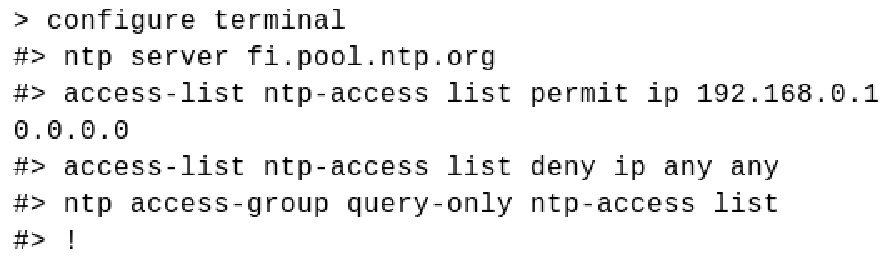
\includegraphics[scale=0.6]{Figures/cli.pdf}
	\caption{Resumen de operaciones en NETCONF.}
	\label{fig:netconf_operaciones}
  \end{figure}


  \subsubsection{Notificaciones}

  Si bien NETCONF está diseñado principalmente para la administración de la configuración de la red mediante las operaciones expuestas anteriormente, existe una poderosa herramienta de monitoreo implementada en el protocolo, llamada notificaciones. La RFC5277 define a las mismas como un servicio de entrega de mensajes asíncronas a los clientes mediante suscripción. Esta característica no es obligatoria para las diferentes implementaciones del protocolo NETCONF. De soportarlo, el servidor deberá comunicar a los clientes dicha característica como una capacidad del servidor en el mensaje \textit{HELLO}.
  \\

  Esta herramienta es similar a las notificaciones en el protocolo \textit{SNMP}, pero tiene la ventaja de que en NETCONF, el cliente puede especificar a qué notificación particular se desea suscribir, lo que permite un monitoreo más flexible. Además, como se mencionó anteriormente, el servidor puede declarar permisos para los diferentes usuarios y sesiones por lo que las notificaciones serán enviadas únicamente a aquellos clientes suscritos y que cumplan con el nivel de acceso requerido por el servidor.
  \\

  La importancia de las operaciones soportadas por el protocolo NETCONF reside en que de esta forma, la configuración de la red puede cambiar de forma activa mediante las operaciones que define el protocolo y reactiva mediante las notificaciones, pudiendo reaccionar ante un cambio en el dispositivo de forma automática.
  \\

  Para finalizar, la figura \ref{fig:netconf_ejemplo} refleja una interacción típica entre cliente y servidor, donde se observa el intercambio de capacidades en los mensajes HELLO, el uso de diferentes operaciones con respuestas RPC y las notificaciones.

  \begin{figure}[htbp]
	\centering
	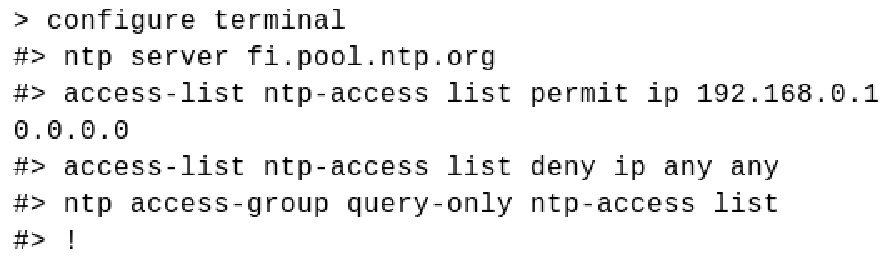
\includegraphics[scale=0.6]{Figures/cli.pdf}
	\caption{Comunicacion entre cliente y servidor NETCONF.}
	\label{fig:netconf_ejemplo}
  \end{figure}

  \subsection{Lenguaje de Modelado YANG}